%%%%%%%%%%%%%%%%%%%%%
% Documento maestro %
%%%%%%%%%%%%%%%%%%%%%
\documentclass[oneside]{fime}


%%%%%%%%%%%%%%%%%%%%%%%%%%%%%%%%%%%%%%%%%%%
% Cargando paquetes y definiendo opciones %
%%%%%%%%%%%%%%%%%%%%%%%%%%%%%%%%%%%%%%%%%%%
% Aquí puedes cargar los paquetes que vas a usar. La clase
% fime ya incluye babel, inputenc, graphicx y los de la AMS.
% Cargar un paquete está a tu libertad (y responsabilidad).

\usepackage{hyperref}
	\hypersetup{breaklinks=true,colorlinks=true,linkcolor=black,citecolor=black,urlcolor=black}
\usepackage[toc, section=chapter, nopostdot]{glossaries}
	\makenoidxglossaries	
	\loadglsentries{Glosario}
	\setglossarystyle{altlist}
\usepackage[numbers, sort&compress]{natbib}
\usepackage{subfig}


%%%%%%%%%%%%%%%%%%%%%
% Definiendo campos %
%%%%%%%%%%%%%%%%%%%%%
\def\titulo{Detección de cancer de piel mediante segmentación semántica}
\def\autor{Mario Alberto Flores Hernández}
\def\matricula{1719126}
\def\grado{Licenciatura en Ingeniería en Mecatrónica}
% En caso de que el grado tenga orientación o especialidad llenar el siguiente
% campo dejando un ESPACIO INICIAL, en caso contrario, dejar vacío
\def\orientacion{}
% Coloca el mes con mayúscula inicial
\def\fecha{Febrero 2021}

\def\asesor{Dra. Satu Elisa Schaeffer}
\def\revisorA{Dr. Romeo Sánchez Nigenda}
\def\revisorB{Dra. Sara Elena Garza Villarreal}
% En el caso de que tu tesis sea de doctorado activa la variable cambiándola a \doctoradotrue
% y define tus otros dos revisores
\newif\ifdoctorado\doctoradofalse
% El visto bueno siempre va
\def\vobo{Dr. Fernando Banda Muñoz}

\addto\captionsspanish{\renewcommand{\listtablename}{Índice de Cuadros}}

%%%%%%%%%%%%%%%%%%%%%%%
% Inicia el documento %
%%%%%%%%%%%%%%%%%%%%%%%
\begin{document}


\frontmatter
\pagestyle{main}

%%%%%%%%%%%%%%%%%%%%%%%%
% Primer portada: UANL %
%%%%%%%%%%%%%%%%%%%%%%%%
\thispagestyle{empty}

\begin{scshape}
\begin{center}
	{\Large \uanl} \\[5mm]
	{\large \fime} \\[5mm]
	{\large \depg}
	\vskip15mm
	
\includegraphics[height=55mm]{uanl}
	\vskip12mm
	\begin{tabular}{p{11cm}}
		\centering
		{\large \titulo}
	\end{tabular}
	\vskip7mm
	{por}\\[7mm]
	{\large \autor}\\[7mm]
        % Si en tu posgrado la tesis no es opcional (como sí lo es en licenciatura), no modifiques esta línea:
	{como requisito parcial para obtener el grado de}\\[3mm]
	\MakeUppercase{\grado}\\
	\orientacion
	\vfill
	\fecha
\end{center}
\end{scshape}

%%%%%%%%%%%%%%%%%%%%%%%%%
% Segunda portada: FIME %
%%%%%%%%%%%%%%%%%%%%%%%%%
\newpage
\thispagestyle{empty}

\begin{scshape}
\begin{center}
	{\Large\uanl} \\[5mm]
	{\large\fime} \\[5mm]
	{\large\depg}
	\vskip16mm
	
\includegraphics[height=50mm]{fime}
	\vskip16mm
	\begin{tabular}{p{11cm}}
		\centering
		{\large \titulo}
	\end{tabular}
	\vskip7mm
	{por}\\[7mm]
	{\large \autor}\\[7mm]
        % Si en tu posgrado la tesis no es opcional (como sí lo es en licenciatura), no modifiques esta línea:
	{como requisito parcial para obtener el grado de}\\[3mm]
	\MakeUppercase{\grado}\\
	\orientacion
	\vfill
	\fecha
\end{center}
\end{scshape}

%%%%%%%%%%%%%%%%%%%%%%%%%%%%%
% Carta del comité de tesis %
%%%%%%%%%%%%%%%%%%%%%%%%%%%%%
\newpage
\thispagestyle{empty}
\enlargethispage{5mm}

{\renewcommand{\baselinestretch}{1.1}\selectfont
\begin{center}\vspace*{-25mm}\hspace*{-10mm}
\begin{minipage}{170.5mm}
\hspace{-1.5mm}
\includegraphics[height=20mm]{uanl}\hfill\raise1mm\hbox{
\includegraphics[height=18.5mm]{fime}}
\hrule\vspace{0.5mm}
\scalebox{.5}{\MakeUppercase{\uanl}}\hfill\scalebox{.5}{\MakeUppercase{\fime}}\medskip
\end{minipage}
\vskip4mm{\sc\large\uanl\\\fime\\[3pt]\depg}\vskip6mm
\end{center}

Los miembros del Comité de Tesis recomendamos que la Tesis <<\titulo>>, realizada por el alumno \autor, con número de matrícula \matricula, sea aceptada para su defensa como requisito parcial para obtener el grado de \grado\orientacion.
\ifdoctorado\vskip10mm\else\vskip8mm\fi

\begin{center}
El Comité de Tesis\\
\ifdoctorado\vskip15mm\else\vskip25mm\fi

\ifdoctorado{%%%
\begin{tabular}{p{37mm}p{21mm}p{12mm}p{21mm}p{37mm}}
	\cline{2-4}
	& \multicolumn{3}{c}{\asesor} & \\
	& \multicolumn{3}{c}{Asesor}  & \\[15mm]
	\cline{1-2} \cline{4-5}
	\multicolumn{2}{c}{\revisorA} & & \multicolumn{2}{c}{\revisorB} \\
	\multicolumn{2}{c}{Revisor}   & & \multicolumn{2}{c}{Revisor}   \\[17mm]
	\cline{1-2} \cline{4-5}
	\multicolumn{2}{c}{\revisorC} & & \multicolumn{2}{c}{\revisorD} \\
	\multicolumn{2}{c}{Revisor}   & & \multicolumn{2}{c}{Revisor}   \\[2mm]
	& \multicolumn{3}{c}{Vo. Bo.} & \\[14mm]
	\cline{2-4}
	& \multicolumn{3}{c}{\vobo}   & \\
	& \multicolumn{3}{c}{Subdirector de Estudios de Posgrado}   & \\ &&&&
\end{tabular}
}\else{%%%
\begin{tabular}{p{37mm}p{21mm}p{12mm}p{21mm}p{37mm}}
	\cline{2-4}
	& \multicolumn{3}{c}{\asesor} & \\
	& \multicolumn{3}{c}{Asesora}  & \\[19mm]
	\cline{1-2} \cline{4-5}
	\multicolumn{2}{c}{\revisorA} & & \multicolumn{2}{c}{\revisorB} \\
	\multicolumn{2}{c}{Revisor}   & & \multicolumn{2}{c}{Revisora}   \\[2mm]
	& \multicolumn{3}{c}{Vo. Bo.} & \\[17mm]
	\cline{2-4}
	& \multicolumn{3}{c}{\vobo}   & \\
	& \multicolumn{3}{c}{Subdirector Académico}   & \\ &&&&
\end{tabular}
}\fi%%%

\vfill

\snnl, \MakeLowercase{\fecha}

\end{center}}


\tableofcontents

\listoffigures
\addcontentsline{toc}{chapter}{Indice de Figuras}

\listoftables
\addcontentsline{toc}{chapter}{Indice de Cuadros}

\chapter{Notaciones}

A continuación se resumen las notaciones usadas a lo largo de este trabajo de tesis, incluyendo el símbolo,  significado y equivalente en el idioma inglés.

\begin{itemize}
    \item $x$, dato de entrada (input).
    \item $y$, dato de salida (output).
    \item $\hat{y}$, salida estimada (estimated output).
    \item $d$, dimensión de entrada (input dimension).
    \item $d_{\rm o}$, dimensión de salida (output dimension).
    \item $n_s$, número de muestras (samples).
    \item $e_i$, entrada del nodo (node input).
    \item $p_i$, peso entre la entrada y el nodo (weight).
    \item $\phi$, función de activación (activation).
\end{itemize}


%Agradecimientos

\chapter{Agradecimientos}
\markboth{Agradecimientos}{}
\coltext{
Aquí puedes poner tus agradecimientos. (No olvides agradecer a tu comité de tesis, a tus profesores, a la facultad y a CONACyT en caso de que hayas sido beneficiado con una beca).
}

%Resumen

\chapter{Resumen}
\markboth{Resumen}{}

{\renewcommand{\baselinestretch}{1.1}\selectfont
{\setlength{\leftskip}{10mm}
\setlength{\parindent}{-10mm}

\autor.

Candidato para obtener el grado de \grado\orientacion.

\uanl.

\fime.

Título del estudio: \textsc{\titulo}.

\noindent Número de páginas: \pageref*{lastpage}.}

%%% Comienza a llenar aquí
\paragraph{Objetivos y método de estudio:}
Desarrollar una herramienta de asistencia para la detección de cáncer de piel utilizando las técnicas mas actuales de visión computacional e inteligencia artificial, se pretende desarrollar mediante \emph{software} y tecnicas de \emph{\gls{seg}} una aplicación que permita introducir una imagen y como resultado obtengamos un mapa de características segmentado en una o más categorías. 

\paragraph{Contribuciones y conclusiones:}
\coltext{}
\newline

\bigskip\noindent\begin{tabular}{lc}
\vspace*{-2mm}\hspace*{-2mm}Firma del asesor: & \\
\cline{2-2} & \hspace*{1em}\asesor\hspace*{1em}
\end{tabular}}



\mainmatter
\pagestyle{fime}


%%% Haz un documento para cada capítulo


\chapter{Introducción}

La piel es considerada el órgano mas grande del cuerpo humano,  y está compuesta por tres capas: \emph{\gls{epidermis}}, \emph{\gls{dermis}} e \emph{\gls{hipodermis}} (figura \ref{fig:skin1_jpg}). La principal función de la piel es proteger al cuerpo de las hostilidades del medio ambiente como la radiación solar y los factores externos como las bacterias, sin embargo también cumple otras funciones importantes aparte de proteger los órganos y los tejidos internos, tales otras funciones son regular nuestra temperatura corporal, registrar sensaciones de presión, frío, calor y es una interfaz para poder sentir e interactuar con lo que tenemos a nuestro alrededor.

\begin{figure}[h!]
    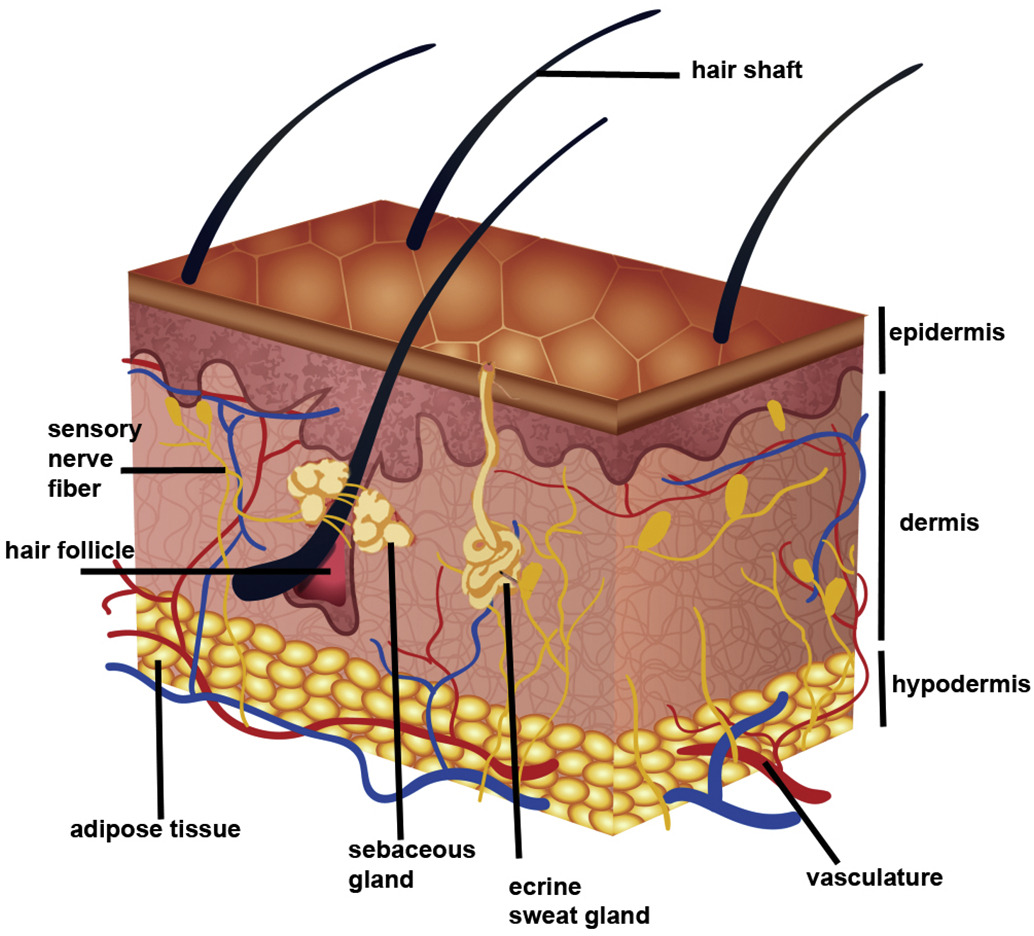
\includegraphics[width=80mm, scale = 0.5]{Figuras/skin_structure1.jpg}
    \centering
    \caption{Ilustración de las capas de la piel y sus apéndices \citep{skin_1}.}
    \label{fig:skin1_jpg}
\end{figure}

Sin embargo, debido a la exposición continua a las radiaciones de la luz, es común desarrollar enfermedades en la piel que afectan la forma en que las células de ésta se reproducen, causando graves daños a nuestra salud que en muchas ocasiones puede llegar a ser letal. Estas anomalías en la piel se denominan como \emph{cáncer de piel}, principalmente en las siguientes tres categorías: cáncer de células basales, cáncer de células escamosas y melanomas \citep{cancer_org}.

\begin{figure}[h!]
    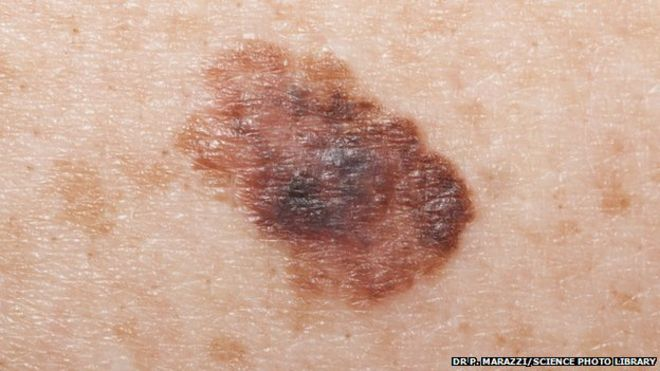
\includegraphics[width=80mm, scale = 0.8]{Figuras/skin_cancer_bbc.jpg}
    \centering
    \caption{Ejemplo de melanoma \citep{cancer_img_1}}
    \label{fig:can_jpg}
\end{figure}
 Su detección temprana es imprescindible para reducir las probabilidades de fallecimiento. Por lo tanto es necesario seguir desarrollando tecnologías que faciliten la detección de este tipo de padecimientos de forma rápida y sencilla que vaya enfocada en aumentar la accesibilidad a dichos diagnósticos y de esta forma reducir la tasa de mortalidad por este padecimiento.

En los últimos años se han logrado muchos avances en cuanto al desarrollo de software inteligente que han permitido un mayor acceso a diferentes servicios, una de estas tecnologías sería la \emph{\gls{rn}}, se trata de una tecnología que tiene la capacidad de \emph{aprender} mediante el úso de datos históricos y funciones de optimización para crear un modelo matemático capaz de predecir, clasificar o recrear datos futuros o desconocidos. Algunos de los sectores que han comenzado a adoptar esta tecnología son: el sector automotriz (piloto automático), el sector de manufactura (optimización de procesos), el sector de entretenimiento (recomendaciones personalizadas), el sector médico (diagnóstico de imágenes). 


\section{Hipótesis}
Es posible clasificar los píxeles en distintas categorías dentro de una imagen gracias a las avances actuales de inteligencia artificial y la técnica de segmentación. Mediante la técnica de \emph{\gls{seg}} es posible crear un reconocedor visual que no solo detecte la presencia y ubicación del elemento a reconocer, sino que, también obtenga otros datos descriptivos del elemento como el tamaño, forma y región que abarca dentro de la imagen.

\section{Objetivos}
Primero en \emph{objetivo General} se habla de manera conceptual la problemática a resolver tales como cuales son las situaciones en las que podemos optimizar la resolución de un problema mediante el uso de la red neuronal, posteriormente en los \emph{objetivos Específicos} se describe de forma puntual los pasos a realizar en el presente trabajo de tésis para llegar al resultado deseado.

El \emph{objetivo general} de este trabajo de tésis es la creación de una aplicación capaz de detectar anomalías en la superficie piel que correspondan a alguno de los tipos de \emph{cáncer de piel} mediante imágenes (basalioma, carcinoma, melanoma), con el uso de la red neuronal de \emph{\gls{seg}} usando como base la librería mencionada en \citet{wu2019fastfcn}. 


El \emph{objetivo específico}, es el implementar un modelo de red neuronal cuya entrada sean imágenes que pueden o no contener la presencia de alguno de los tipos de cáncer de piel comunes, y como salida del modelo se obtenga un mapa de características donde de haber presencia de el cáncer este se distinga mediante una región colorada en el espacio que abarca. El modelo debe cumplir con las siguientes características:

\begin{itemize}
    \item El modelo debe ser capaz de trabajar con imágenes a color o en blanco y negro.
    \item El modelo debe contar con una función capaz de evaluar la precisión.
    \item El modelo debe contar con un algoritmo capaz de optimizar la precisión.
    \item El modelo debe ser capaz de segmentar correctamente imágenes no usadas en los datos de entrenamiento.
\end{itemize}

La gráfica a continuación representa el dato de entrada (izquierda) y el resultado esperado en la salida del modelo (derecha):

\begin{figure}[h!]
    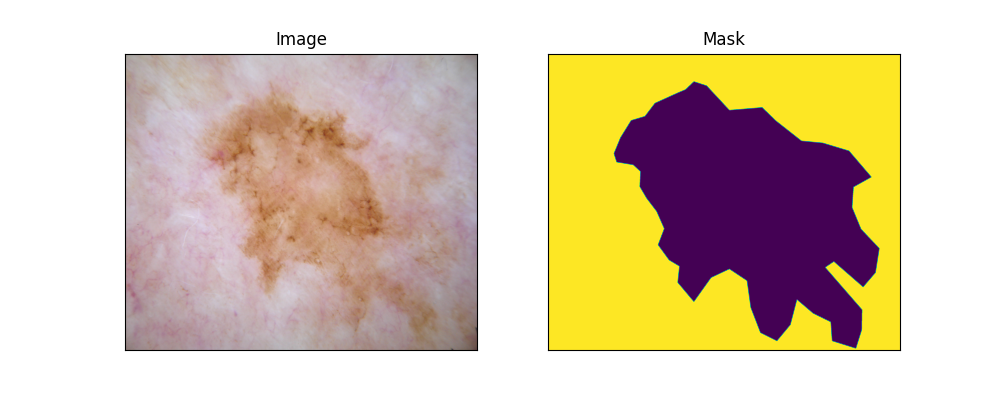
\includegraphics[width=150mm]{Figuras/plot_masks.png}
    \centering
    \caption{}
    \label{fig:desired}
\end{figure}

\section{Estructura de la Tesis}

A continuación se dá una breve descripción sobre los capítulos que se verán a continuación en este documento.

En el capítulo 2 se habla sobre los antecedentes relacionados al presente trabajo de tesis, primero se empieza definiendo la naturaleza del problema con el que se pretende tratar, después algúnos conceptos clave que serán necesarios para la comprensión de la implementación propuesta. 

En el capítulo 3 se habla sobre el estado del arte en cuanto a las redes neuronales, cuales son los avances en los últimos años y que ventajas tenemos ahora comparado al avance que se tenía cuando experimentos fueron realizados.

En el capitulo 4 se describe de forma estadística los datos que serán utilizados para realizar el experimento, tomando en cuenta la distribución de los pixeles en distintas regiones de la imagen, entre otros parámetros. 

En el capítulo 5 se detalla el proceso de implementación, primero se describirán las características del hardware, se describe la arquitectura del modelo y las transformaciones por las que pasará la imagen y luego se hará una comparativa con distintos modelos de redes neuronales para comparar tiempo de entrenamiento, precisión y resultado.

Finalmente, en el capítulo 6 se exponen los resultados obtenidos de la implementación del producto científico en el capítulo anterior, así como un análisis y conclusión final sobre los valores obtenidos en precision y tiempo de entrenamiento. 

\chapter{Antecedentes}
En este capítulo se introducen de forma teórica los conceptos relacionados a los tipos de cáncer y las redes neuronales, primero se define que es el \emph{cáncer de piel}, cuales son los factores que influyen en el desarollo de este padecimiento, los tipos de cáncer y las diferencias entre estos. Después algunos conceptos relacionados con las redes neuronales necesarios para un entendimiento sólido del \emph{aprendizaje profundo}, tales como los elementos clave que conforman a la red neuronal, la manera en la que esta evalúa su precisión, y el algoritmo de optimización.

\section{Cáncer de Piel}
El \emph{cáncer de piel} es una enfermedad que suele relacionarse con la aparición de lunares o manchas que no se encontraban previamente, se pueden manifestar como manchas oscuras o rojizas, bultos y/o escamas en la superficie de la piel y afecta a todos los tonos de la piel por igual. Esta enfermedad se desarrolla principalmente en partes del cuerpo expuestas al sol, sin embargo también se puede desarrollar en partes que no suelen exponerse. Algunos factores como la exposición a los rayos ultravioletas (UV), el uso de sustancias como el tabaco o el envejecimiento son factores correlacionados con la aparición del \emph{cáncer de piel}, existen dos factores de envejecimiento y se dividen en dos grupos: 

\begin{itemize}
    \item Factores intrínsecos 
    \item Factores extrínsecos 
\end{itemize}

Los factores \emph{intrínsecos} son aquellos que suceden de forma interna en la piel, un ejemplo de esto es el envejecimiento cronológico, el cual es un proceso natural que consiste en degradación del colágeno, la elastina y el adelgazamiento de la epidermis debido al envejecimiento celular al paso de los años y de el efecto de algunas hormonas.

Los factores \emph{extrínsecos} son aquellos que suceden de forma agena al organismo, como es el caso del \emph{foto-envejecimiento} el cual sucede cuando nos encontramos expuestos a los rayos ultravioletas (UV). Este factor de envejecimiento genera lesiones en las cadenas de ácido desoxirribonucleico (ADN) debido a la oxidación y afecta la regeneración de celulas, al sistema inmune y a la forma en la que se regula la pigmentación \citep{skin_aging}.

\subsection{Tipos de Cáncer de Piel}
Existe una gran variedad de tipos de \emph{cáncer de piel}, sin embargo son cuatro tipos los que destacan por tener una mayor incidencia:

\begin{itemize}
    \item melanoma
    \item cáncer de piel no melanoma
    \item carcinóma de celulas basales
    \item carcinóma epidermoide de piel
\end{itemize}

\coltext{Necesito mas referencias sobre esta información}

\section{Redes Neuronales}

Hasta hace algunos años el desarollo de aplicaciones de software solía realizarse de una forma robústa, por ejemplo, si desearamos desarrollar una aplicación de reconocimiento de imagenes de la forma tradicional ,sin embargo es posible resolver los mismos problemas de una forma distinta mediante el uso de los datos históricos. Algunos de los puntos clave que conforman una red neuronal son los siguientes:

\begin{itemize}
    \item Datos: Se debe determinar la naturaleza y la dimensión de los datos que entrarán al modelo.
    \item Modelo: Se debe crear un sistema que transforme los datos de entrada, en la salida deseada.
    \item Evaluación: El modelo debe tener la capacidad de evaluar su precisión.
    \item Optimización: El modelo debe contar con un algoritmo que optimice la precisión.
\end{itemize}

\subsection{Imágenes como Datos}
Las \emph{imágenes} se pueden definir como una matriz de $\mathbf{m}$ x $\mathbf{n}$ x $\mathbf{1}$ pixeles en el caso de las imágenes de un solo canal (blanco y negro) y de $\mathbf{m}$ x $\mathbf{n}$ x $\mathbf{k}$, donde $\mathbf{k}$ es igual al numero de canales que tenga la imagen, siendo tres en el caso de imágenes a color (RGB), es importante definir si las imágenes ingresarán al modelo a color o en blanco y negro debido a que esto define el numero de nodos de entrada del modelo, ya que para cada pixel debe corresponder un nodo de entrada y en el caso de imágenes a color también deberá tener un número de capas de nodos igual al número de canales que tenga la imagen. 

\subsection{Modelo}
Un \emph{modelo} se puede definir como el bloque intermedio entre los datos de entrada (input) y los datos de salida (output), es el sistema encargado de transformar los datos y consta de los siguientes componentes:

\begin{itemize}
    \item Capa de nodos de entrada (Input nodes): Se trata de la primera capa del modelo, en el caso de imágenes a cada pixel le corresponde un nodo de entrada. Estos nodos deben tener las mismas dimensiones que las imagenes de entrada.
    \item Capa de nodos ocultos (Hidden nodes): Las dimensiones de estos nodos pueden ser diferentes a los de entrada y tener varias capas ocultas, sin embargo esto puede afectar la complejidad y precisión del modelo.
    \item Capa de nodos de salida (Output nodes): Esta es la capa de salida del modelo, las dimensiones de la capa de salida determinan las dimensiones del dato resultante.
    \item Función de activación (Activation): Se trata de una función dentro de cada nodo que interactúa con el valor entrante y se multiplica por el peso.
    \item Pesos (Weights): Se trata de un valor entre el nodo de la capa actual y el nodo siguiente inicializado de forma aleatoria y después ajustado por un algoritmo para aproximar la salida al valor real.
    \item Bías (Bias): Se trata de un valor constante que se suma al resultado de la función de activación y el peso, de esta forma se puede ajustar que tan fácil o difícil es activar un nodo.
\end{itemize}

\subsection{Evaluación y Optimización}
Para realizar el proceso de \emph{aprendizaje} del modelo, primero se debe evaluar cuál es el estado actual de las predicciones. Para esto es necesario evaluar que distancia existe entre el valor predicho y el valor real, esto se puede lograr mediante una \emph{función de pérdida} que se encargue de determinar que tanta diferencia (loss) existe en las estimaciones del modelo con los pesos actuales.

Un ejemplo de la función de pérdida es el de la función logarítmica del costo (log-likelihood), como se muestra a continuación:

$l(\mathbf{y}, \hat{\mathbf{y}}) = - \sum_{j=1}^q y_j \log \hat{y}_j$ 

Donde: 
\begin{itemize}
    \item $q$: Representa el número de clases entre las debe cuales predecir.
    \item $y_j$: Representa valor real.
    \item $\hat{y_j}$: Representa valor estimado por el modelo.
    \item $j$: Representa la posición en el indexado de las clases.
\end{itemize}

Ya que se tiene calculada la pérdida del modelo en su configuración actual, es necesario actualizar el valor de todos los pesos dentro del modelo para poder acercarnos al valor real. Aquí es donde se requiere un algoritmo que primero determine si el peso de cada nodo debe aumentar o disminuir, y después de determinar la dirección realizar un ajuste antes de volver a evaluar el modelo.

Para esto existe el algoritmo de \emph{gradiente descendiente}, comienza en un punto inicial y repetidamente da un paso hacia la dirección opuesta del gradiente en cada punto y así minimizar el \emph{costo}. A continuación se representa la forma del algoritmo:

\begin{tabbing}
    \hspace*{1.5in} \= \hspace*{0.7in} \= \hspace*{.25in} \= \hspace*{.25in} \= \hspace*{.25in} \=\kill
    \>{\bf Para} $k=0,1,2 \dots n$ {\bf Realiza } \\
    \>\> $g_k \leftarrow \nabla f(x_k)$ \\
    \>\> $x_{k+1} \leftarrow x_k - t_k g_k$ \\
    \>{\bf Termina} \\
\end{tabbing}


\chapter{Estado del Arte}
A continuación se hará un estudio de los trabajos relacionados con el problema señalado en este trabajo de tesis y también con el método propuesto para solucionarlo.

\section{Trabajos Similares}

\section{Área de Oportunidad}


\chapter{Descripción de los Datos}

\chapter{Implementación de la Solución}

\chapter{Resultados}



\appendix
%%% Haz un documento para cada apéndice, si es que tienes

\backmatter
\pagestyle{main}

% Aquí va la bibliografía, puedes usar el entorno de LaTeX (thebibliography)
% o la herramienta BibTeX. En caso de que optes por BibTeX, puedes usar
% alguno de los archivos de estilo (mighelbib.bst o mighelnat.bst) incluidos
% en el paquete, cuyos diseños armonizan con el diseño de tesis provisto por
% fime.cls. Para muestra, basta un botón:

\printnoidxglossary[sort=word]
\bibliographystyle{mighelnat}
\bibliography{MiBiblio}
\addcontentsline{toc}{chapter}{Bibliografía}

\label{lastpage}
%Autobiografia

\chapter*{Resumen autobiográfico}
\thispagestyle{empty}

\begin{center}
\autor

Candidato para obtener el grado de\\
\grado\\
\orientacion\bigskip

\uanl\\
\fime\bigskip

Tesis:\\
\textsc{\large\titulo}
\end{center}\bigskip

%Aquí va tu historia
Nací el 4 de junio de 1997 en la ciudad de Monterrey, Nuevo León. Hijo del Sr. Mario Alberto Flores Rosales y la Sra. Patricia Hernández Romero. Comencé mis estudios de Ingeniería en Mecatrónica en agosto de 2014 en la \uanl, en marzo de 2019 llevé a cabo el diplomado de Innovación Biomédica.


\end{document}

